\begin{pastexam}[label={px:gk3-098-ds-01}]{高考三級資訊處理 98 年 第一題}
（申論；25 分）

二元樹（binary tree）
\begin{itemize}[leftmargin=2.2em]
\item[㈠] 有一個二元樹（binary tree）的中序走訪（inorder traversal）順序為 ABCDEFGHI，它的後序走訪
（postorder traversal）順序為 BACFEIHGD，其中每個英文字母代表一個節點。請畫出此二元樹。（6 分）
\item[㈡] 上述二元樹的前序走訪（preorder traversal）順序為何？（6 分）
\item[㈢] 在二元搜尋樹（binary search tree）中，那一個走訪順序（前序、中序或後序）正好為排序好的情況？
原因何在？（本小題未寫明原因者，不給分）（6 分）
\item[㈣] 如何利用線性掃瞄方式，判斷一個前序運算式（prefix expression）是否合法？（7 分）
\end{itemize}
\end{pastexam}

\begin{pastsoln}
答案：㈠ 樹如下圖；㈡ DCABGEFHI；㈢ 中序；㈣ 用一個「還缺幾個運算元」的計數器，由左往右
掃一次。 ㈠㈡㈢ 屬第~7~章，㈣ 屬第~6~章（運算式）。

\textbf{㈠} 用中序加後序重建（資結書第~7.4~節）：後序的最後一個是根，在中序裡找到它，左邊是左子樹、
右邊是右子樹；兩邊的節點數決定後序怎麼切。
\begin{center}
\small
\begin{tabular}{llll}
\toprule
中序 & 後序 & 根 & 左子樹／右子樹（中序） \\
\midrule
ABCDEFGHI & BACFEIHGD & D & ABC ／ EFGHI \\
ABC & BAC & C & AB ／ 空 \\
AB & BA & A & 空 ／ B \\
EFGHI & FEIHG & G & EF ／ HI \\
EF & FE & E & 空 ／ F \\
HI & IH & H & 空 ／ I \\
\bottomrule
\end{tabular}
\end{center}
第一列：D 左邊有 3 個（ABC），所以後序的前 3 個 BAC 是左子樹、接下來 5 個 FEIHG 是右子樹。 其餘
各列同理。 得到的樹：
\begin{center}
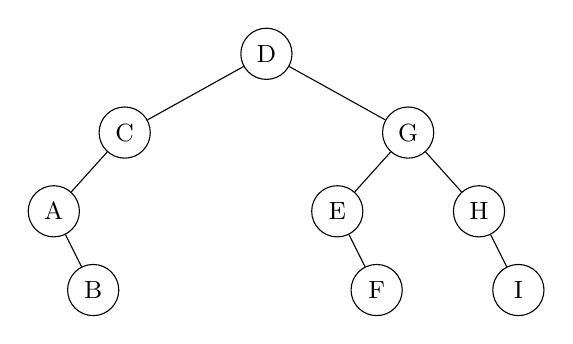
\begin{tikzpicture}[v/.style={circle,draw,minimum size=6.5mm,inner sep=0pt,font=\small},
    level distance=10mm, level 1/.style={sibling distance=36mm},
    level 2/.style={sibling distance=18mm}, level 3/.style={sibling distance=10mm}]
\node[v] {D}
  child {node[v] {C}
    child {node[v] {A} child[missing] {} child {node[v] {B}}}
    child[missing] {}}
  child {node[v] {G}
    child {node[v] {E} child[missing] {} child {node[v] {F}}}
    child {node[v] {H} child[missing] {} child {node[v] {I}}}};
\end{tikzpicture}
\end{center}
檢查：這棵樹的中序是 ABCDEFGHI、後序是 BACFEIHGD，和題目一樣。 中序加後序（或中序加
前序）決定唯一的一棵二元樹，所以這就是答案。

\textbf{㈡} 前序（根、左、右）：D，接著左子樹 C A B，再右子樹 G E F H I。 答案是
\textbf{DCABGEFHI}。

\textbf{㈢} \textbf{中序}。 二元搜尋樹的性質：任一節點 $x$，左子樹的鍵都 $\le x.\mathit{key}$，右
子樹的鍵都 $\ge x.\mathit{key}$（資結書第~9~章）。 中序對每個節點都是「先整個左子樹，再自己，再整個
右子樹」，對樹高做歸納：左、右子樹的中序各自由小到大（歸納假設），左子樹的鍵都不大於 $x$、右子樹的鍵
都不小於 $x$，接起來就是由小到大。 前序、後序把根放在最前或最後，根一般不是最小（最大）值，所以不會
是排好的，例如根是 $2$、左右是 $1$、$3$ 的樹，前序 $2, 1, 3$、後序 $1, 3, 2$ 都沒有排好。

\textbf{㈣} 設運算子都是二元運算子。 前序式的文法是「運算式 $=$ 運算元，或 運算子 運算式 運算式」。 由
左往右讀時，用 $\mathit{need}$ 記「還要再讀到幾個完整的運算式」：一開始 $\mathit{need} = 1$（整個式子
本身）；讀到運算元，填掉一個位置，$\mathit{need}$ 減 $1$；讀到運算子，它本身填掉一個位置、又開出兩個
位置，$\mathit{need}$ 加 $1$。 合法的條件是：讀每個符號之前 $\mathit{need} \ge 1$（否則式子已經結束、
後面多出符號），讀完時 $\mathit{need} = 0$（否則運算元不夠）。
\begin{pseudo}[unbreakable]{判斷前序式是否合法}
\Function{Prefix-Valid}{$s, n$} \Comment{$s[1..n]$ 是符號序列}
    \State $\mathit{need} \gets 1$
    \For{$i \gets 1$ \To $n$}
        \If{$\mathit{need} = 0$}
            \State \Return \FALSE \Comment{式子已經完整，後面還有符號}
        \EndIf
        \If{$s[i]$ 是運算子}
            \State $\mathit{need} \gets \mathit{need} + 1$
        \Else
            \State $\mathit{need} \gets \mathit{need} - 1$
        \EndIf
    \EndFor
    \State \Return $\mathit{need} = 0$
\EndFunction
\end{pseudo}
例子：$* + a\, b\, c$：$\mathit{need}$ 依序為 $1 \to 2 \to 3 \to 2 \to 1 \to 0$，合法；$+ a$：讀完
$\mathit{need} = 1$，不合法（少一個運算元）；$+ a\, b\, c$：讀 $c$ 之前 $\mathit{need} = 0$，不合法
（多一個運算元）。

為什麼對：$\mathit{need}$ 正好是「目前讀過的前綴，要再接幾個完整運算式才能補成一個運算式」。 每個前綴
都可以補完（$\mathit{need} \ge 1$）、整串剛好補完（$\mathit{need} = 0$），就是文法推得出來的字串；
中途變成 $0$ 表示某個前綴已經是完整運算式，整串就多了符號。 掃一次、每個符號 $O(1)$，時間 $O(n)$、
額外空間 $O(1)$。 也可以由右往左掃、用堆疊（資結書第~6.3~節）：運算元推入，運算子彈出兩個、推回一個，
彈出時不夠兩個或最後堆疊裡不是恰好一個就不合法，同樣是 $O(n)$。
\end{pastsoln}
